\documentclass[a4paper,11pt]{scrbook}

\usepackage{swThesis}
\usepackage{amsmath}
\usepackage{lipsum}
\usepackage{standalone}
\usepackage{pdfpages}
\standalonetrue

\bibliography{bibliography}

% Figures
\graphicspath{./figs}

\begin{document}

\chapter{Appendix}

\appendix

This appendix contains journal articles and a book chapter published during my PhD.

\begin{enumerate}
    \item ``Next Generation Phenotypic Screening''; S.J Warchal, A Unciti-Broceta, N.O Carragher; Future Medicinal 
Chemistry; 2016; DOI:10.4155/fmc-2016-0025
    \item ``Development of the Theta Comparative Cell Scoring Method to Quantify Diverse Phenotypic Responses Between 
Distinct Cell Types''; S.J Warchal, J.C Dawson, N.O Carragher; Assay and Drug Development Technologies; 2016; 
DOI:10.1089/adt.2016.730
    \item ``Data-analysis strategies for image-based cell profiling''; J.C Caicedo, S Cooper, F. Heigwer, S.J Warchal, 
P Qui, C Molnar, A Vasilevich, J.D Barry, H.S Bansal, O Kraus, M Wawer, L Paavolainen, M.D Herrmann, M Rohban, J Hung, 
H Hennig, J Concannon, I Smith, P Clemons, S Singh, P Rees, P Horvath, R Linington, A.E Carpenter; Nature Methods; 
2017; doi:10.1038/nmeth.4397
    \item ``High-Dimensional Profiling: The Theta Comparative Cell Scoring Method''; S.J Warchal, J.C Dawson, N.O 
Carragher; Phenotypic Screening: Methods and Protocols, Methods in Molecular Biology; 2018; 
DOI:10.1007/978-1-4939-7847-2\_13
\end{enumerate}

Publication submitted but not included in the appendix:

\begin{enumerate}
    \item ``Evaluation of Machine Learning Classifiers to Predict Compound Mechanism of Action when Transferred Across 
Distinct Cell-Lines''; S.J Warchal, J.C Dawson, N.O Carragher; SLAS Discovery; \textbf{under review}
\end{enumerate}

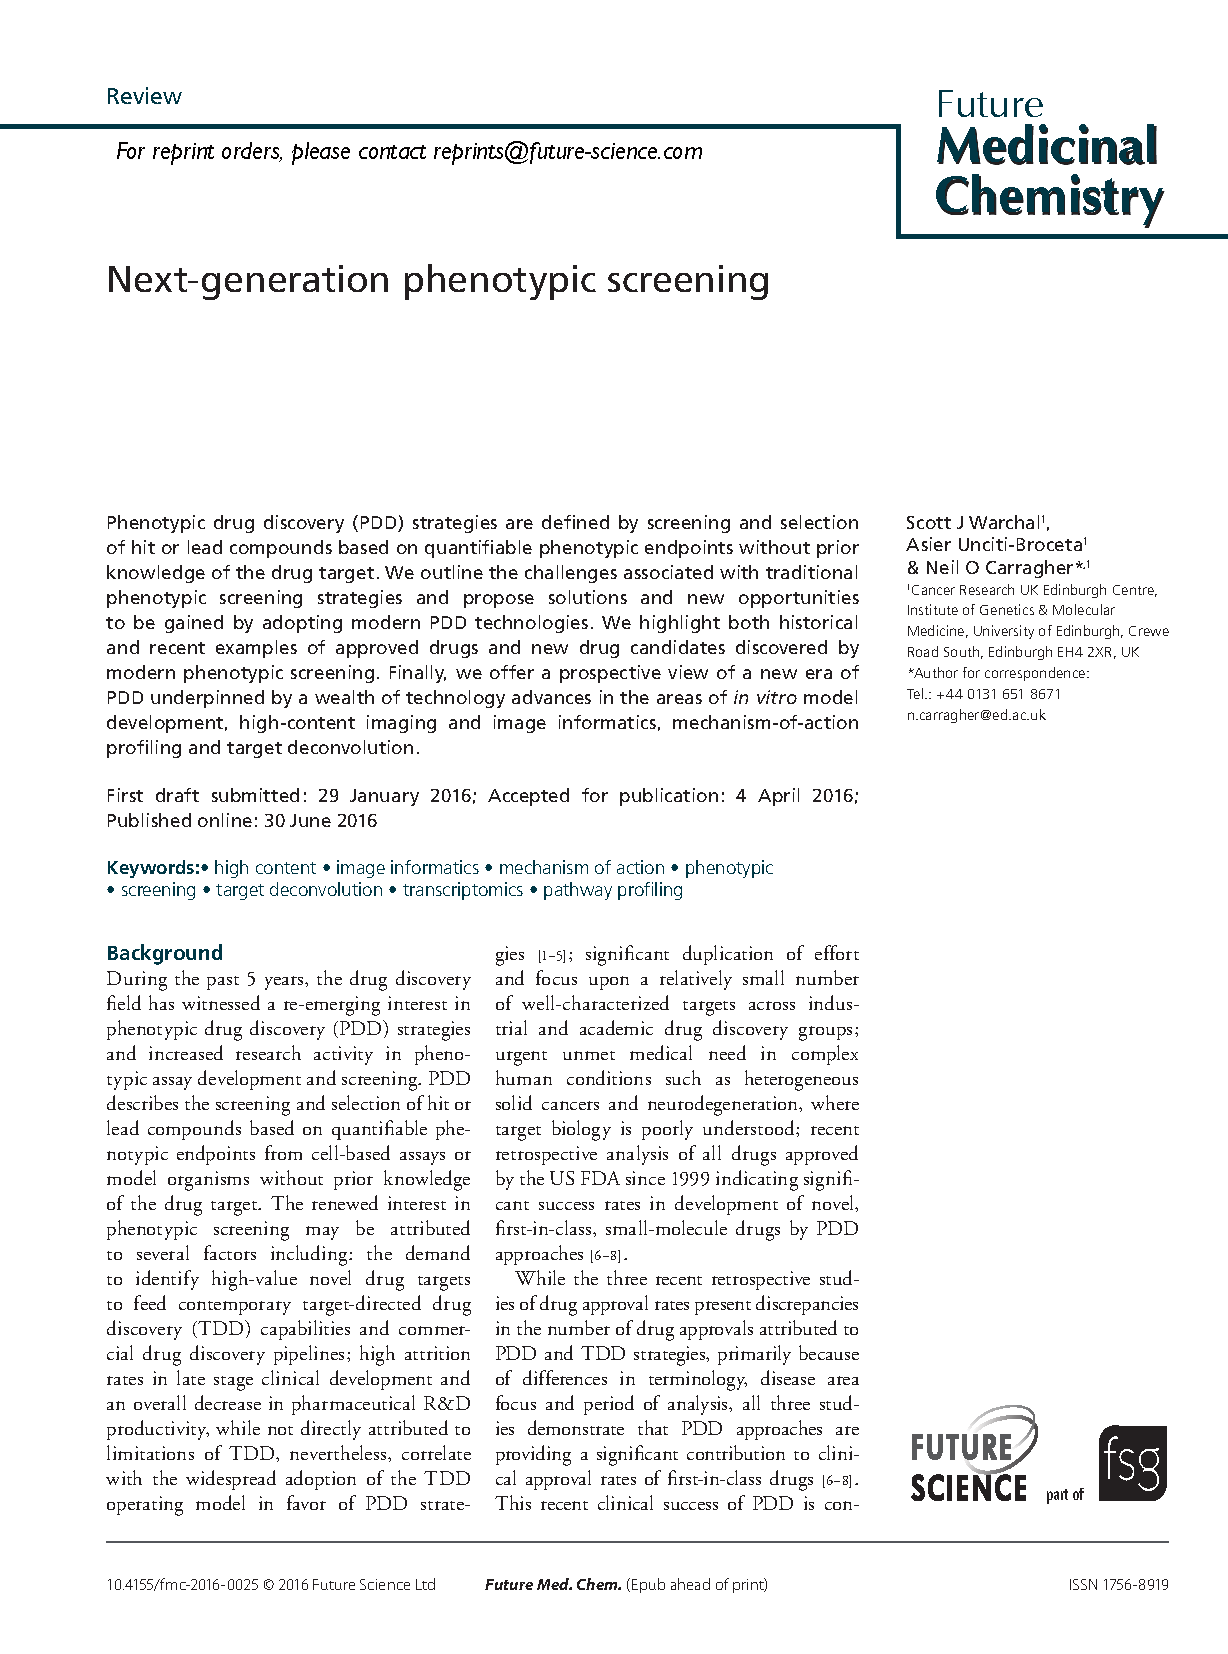
\includepdf[pages=-,scale=0.9]{2016nextgen.pdf}
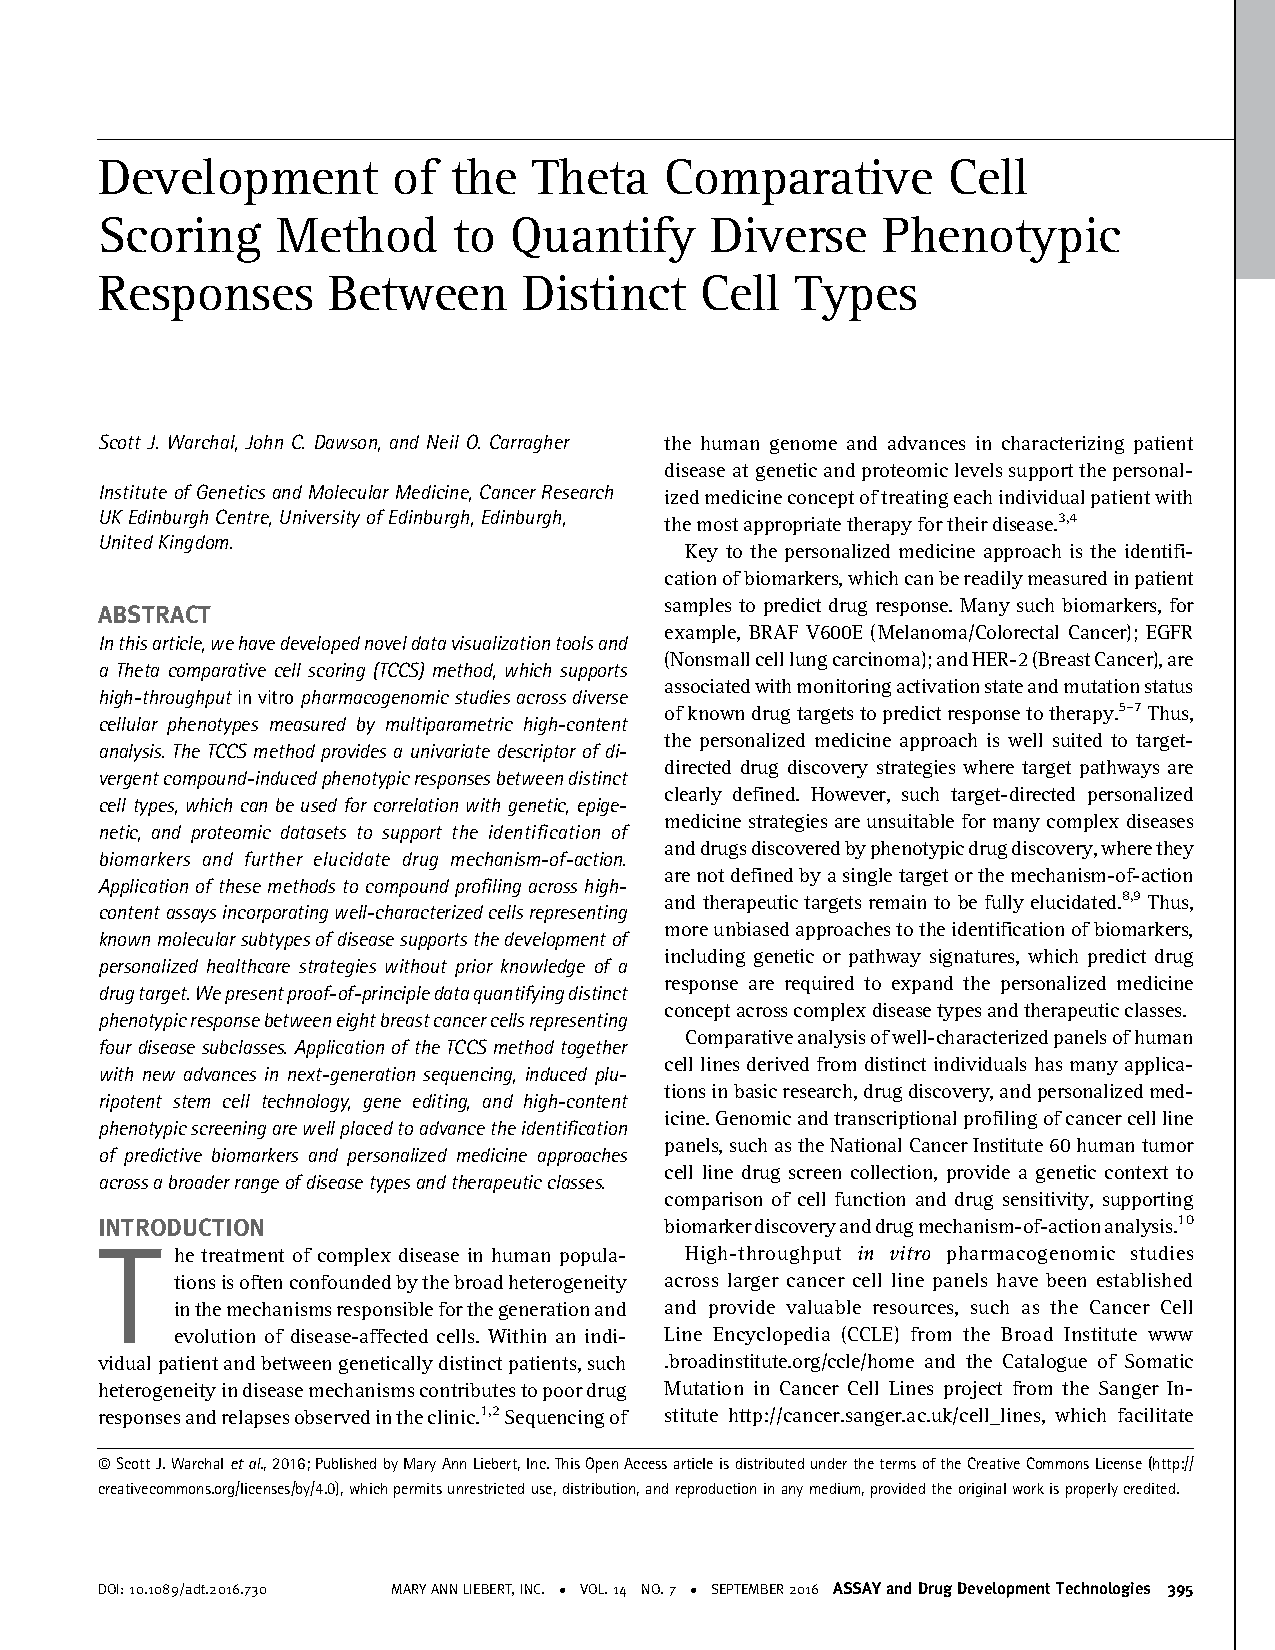
\includepdf[pages=-,scale=0.8]{2016tccs.pdf}
\includepdf[pages=-,scale=0.9]{2017nmeth.pdf}
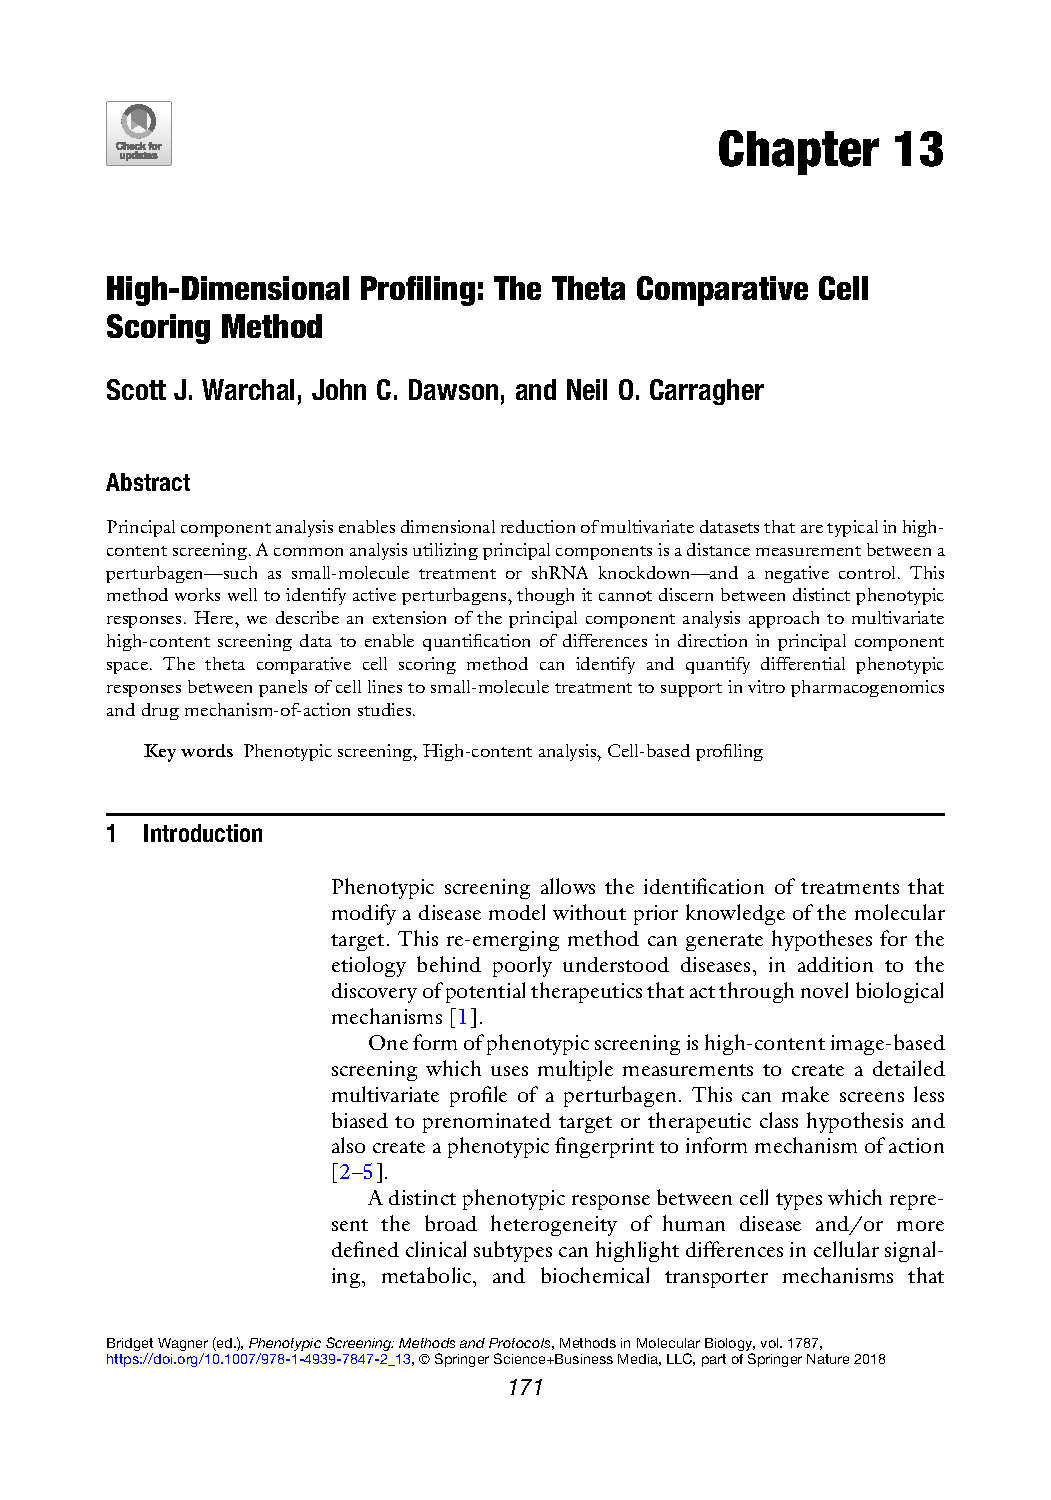
\includepdf[pages=-,scale=0.9]{2018tccs.pdf}

\section*{CellProfiler features}

\begin{table}[H]
    \begin{tiny}
        \input{08_appendix/measured_features.txt}
    \end{tiny}
\end{table}

\begin{table}[H]
    \begin{tiny}
        \input{08_appendix/measured_features_2.txt}
    \end{tiny}
\end{table}

\begin{table}[H]
    \begin{tiny}
        \input{08_appendix/measured_features_3.txt}
    \end{tiny}
\end{table}
\end{document}
